\section{Pré-étude}


\subsection{ Diagramme de contexte }

Le système ATC étudié ici interagit avec quatre acteurs externes qui permettent de définir la frontière du système : 

\begin{itemize}
	\item Les compagnies aériennes,
	\item Les pilotes,
	\item Les aéronefs,
	\item Le service météo. 
\end{itemize}

Les acteurs environnementaux n'ont pas été pris en compte. La référence GPS de synchronisation est considérée comme appartenant au système

	\begin{figure}[H]
	\begin{center}	
		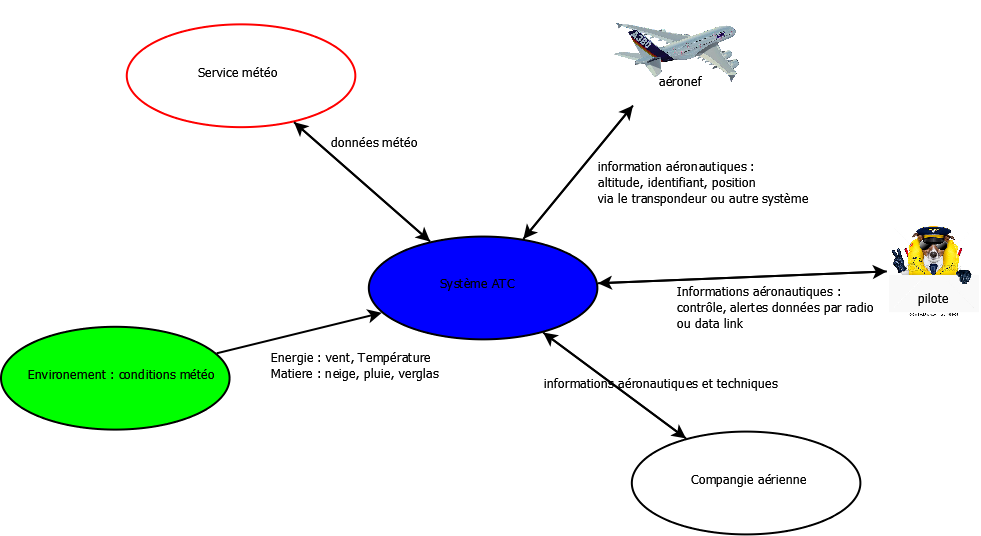
\includegraphics[scale=0.35]{images/ctx}
		\caption{Diagramme de contexte du système ATC}
		\label{ctx}
	\end{center}
\end{figure}

\subsection{ Description graphique du méta-modèle }

Les fonctions, les items et les composants sont les principaux éléments du méta modèle de la  figure \ref{meta}. En particulier, une fonction peut recevoir en entrée, ou fournir en sortie, un item information ou être déclenchée par un item signal électrique. La classe Requirement est intéressante dans le sens où elle permet de vérifier que les exigences sont toutes "mapées" avec un fonction qu'elle spécifie. 

\begin{figure}[H]
	\begin{center}	
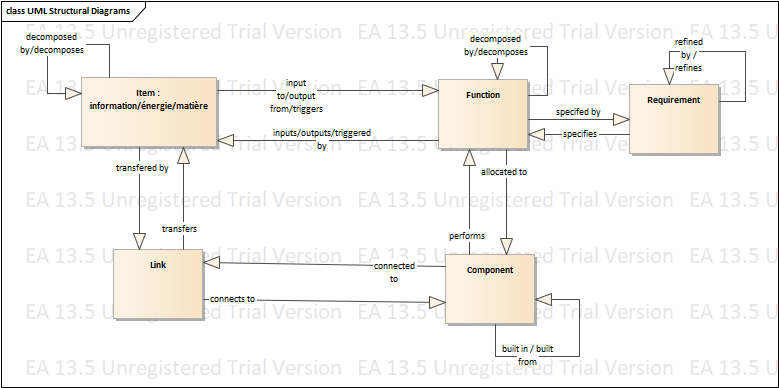
\includegraphics[scale=0.50]{images/meta_modele}
\caption{meta modèle Vitech core}
\label{meta}
	\end{center}
\end{figure}


\subsection{ Données manipulées }

Les données manipulées sont les suivantes :
\begin{itemize}
	\item L'identifiant issu du plan de vol ou d'un radar secondaire,
	\item La position de l'aéronef.
\end{itemize}

La position d'un aéronef vu par un radar primaire ne donne que la distance et l'azimut. Les radars secondaires donnent en outre l'altitude et l'identifiant de l'appareil. Les positions radar doivent être converties en longitude/latitude WGS84 pour pouvoir être affichées. Ce dernier point n'a pas été pris en compte explicitement dans le modèle. En outre, le modèle CORE
ne distingue pas clairement entre position 2D des radars primaires et 3D des radars secondaires ; les fonctions de traitements spécifiques, ainsi que d'autres fonctions, ont été supprimées pour limiter la taille des  graphes hiérarchiques et EFFBD. Ceci constitue un écart par rapport au cahier des charges de l'énoncé mais reste dans l'esprit de l'exercice.
